\chapter{Discriminative $k$-mers}

\section{Definition and characteristics}

A common way of distinguishing between haplotypes is through single nucleotide polymorphisms (or SNPs for short)\cite{snp}. If we were to align the two haplotypes, SNPs would mark the positions in the alignment where the haplotypes differ by a single base (be it a substitution, deletion or insertion)

\begin{figure}
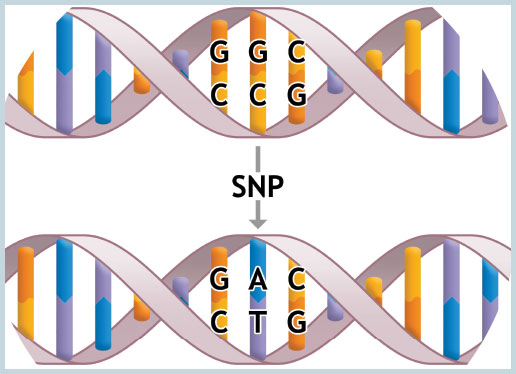
\includegraphics[width=200bp]{figures/snps.jpg}
\caption{SNP\cite{snp_img}}
\label{fig:k_too_low}
\end{figure}

During the sequencing, the SNPs are captured in the “context” of their surrounding bases by $k$-mers - a window of $k$ consecutive bases. If we choose $k$ large enough that a chance of two identical $k$-mers occurring in both haplotypes by sheer chance (excluding repeats that occur naturally) is negligible, we could expect each SNP to be captured by up to $k$ $k$-mers. Thanks to the $k$-mers being unique, the reverse would also be true - every such $k$-mer uniquely identifies certain SNPs. Therefore, for each haplotype we expect a set to exist consisting of $k$-mers that do not occur in the other haplotype. We call such $k$-mers discriminative.

For purposes of $k$-mer counting we use the notion of a canonical $k$-mer. A canonical $k$-mer deterministically represents both a $k$-mer and its reverse complement, and is usually computed as a lexicographic minimum of the two. Usage of canonical $k$-mers is necessary, as reads can originate from any of the two strands, yet we want to capture SNPs regardless of the strand we operate on.

Thanks to having a high coverage in the read data set, discriminative $k$-mers can be differentiated from the rest by computing a histogram of all $k$-mers contained in the reads. Since discriminative $k$-mers occur in only one haplotype, while the remaining $k$-mers occur in both, assuming that all the haplotype regions were amplified uniformly we can expect to find two peaks: one with the $x$ value close to the coverage, and one with a value close to the coverage divided by two. The $k$-mers that occur at half the coverage have a high probability of being discriminative. Thus, we can obtain a set of discriminative $k$-mers by collecting those which can be found in the leftmost peak of such histogram.


\section{Determining the value of $k$}

The first step in obtaining the discriminative $k$-mer is the selection of the right $k$ value.
At first glance it might seem like choosing a very high $k$ would yield good results - after all, we want our $k$-mers to be unique within a haplotype and a longer $k$-mer is less likely to occur by chance. However, we have to take into account sequencing errors which will become more pronounced the longer our $k$-mers are. Setting the value of $k$ too high can potentially lead to a scenario, where many $k$-mers get pushed into the low-occurrence side of our histogram, because they frequently overlap regions in reads affected by sequencing errors. Setting $k$ too high is also detrimental to performance, as each incrementation has the potential of growing the set of $k$-mers we need to track.

\begin{figure}
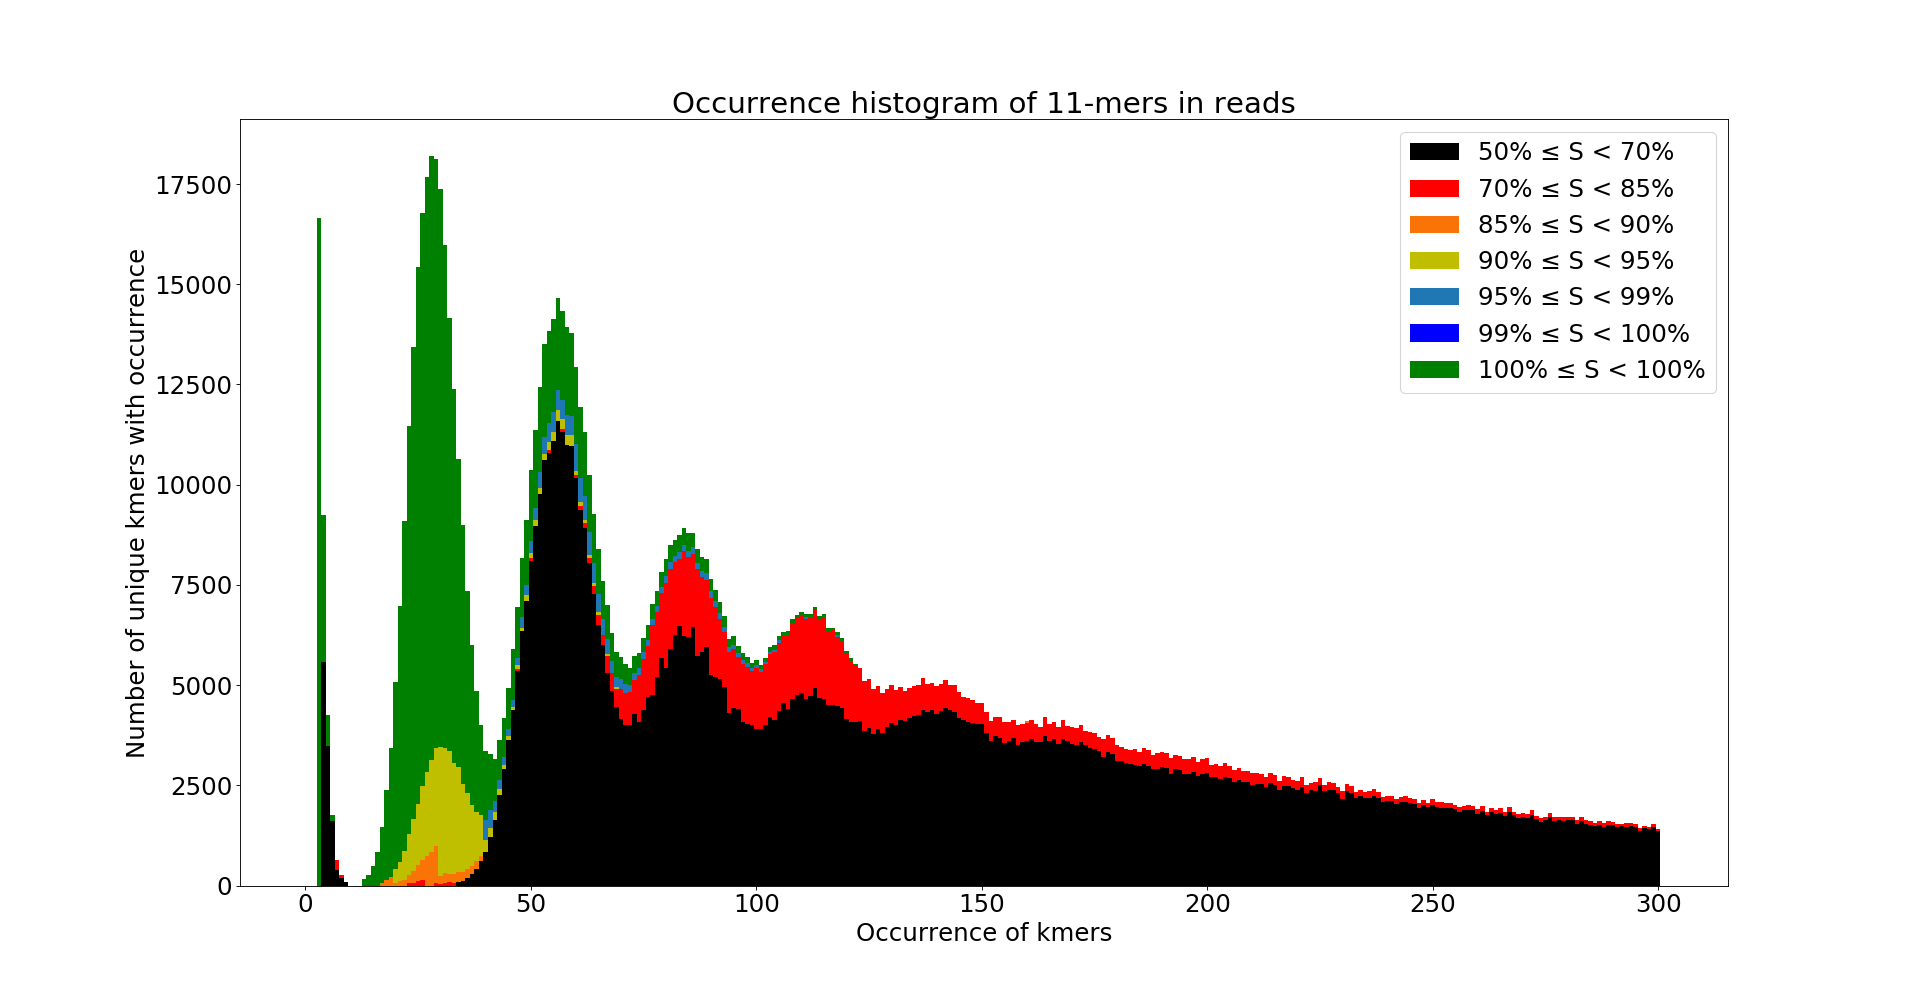
\includegraphics[width=400bp]{figures/k_too_low.png}
\caption{$k$-mer histogram of EIL30 dataset with too small k value. Peaks on the right represent $k$-mers that occur more than once in one haplotype}
\label{fig:k_too_low}
\end{figure}

We choose an empirical approach of choosing $k$ that depends on availability of high-quality reads, such as those obtained from Illumina technology. In the hypothetical case of perfect sequencing, the number of unique $k$-mers found in the reads would be at most equal to the true number of $k$-mers in the genome. Sequencing errors however cause new $k$-mers to emerge. Using high-quality reads such as Illumina alleviates this problem. We can therefore determine a good value of k by trying incrementally higher values and halting whenever the rate of increase of the number of $k$-mers reaches a set threshold. The algorithm can be written as follows:

\begin{figure}[H]
\lstset{language=Python}
\begin{lstlisting}[basicstyle=\small]
def get_unique_kmer_length():
    k = 11
    previous_count = count_kmers(k)
    while k < 33:
        next_count = count_kmers(k + 2)
        if difference(previous_count, next_count) < threshold:
            return k
        previous_count = next_count
        k += 2
    return k
\end{lstlisting}
\caption{Algorithm for determining }
\label{fig:unique_k_size}
\end{figure}

\textit{Note: odd values of k are used frequently, since odd $k$-mers cannot be the mirror images of their complement. We limit the k value by 32, since we represent $k$-mers succinctly by 64 bit integers.}

In order to count the number of $k$-mers quickly and without using large amounts of memory, we use the HyperLogLog algorithm\cite{flajolet2007hyperloglog}. The threshold we set as a halting condition of our algorithm is a 20\% increase in the count of $k$-mers.

For the EIL30 dataset, the determined value of $k$ is 19. Relevant histogram is shown on figure \ref{fig:k19}

\begin{figure}
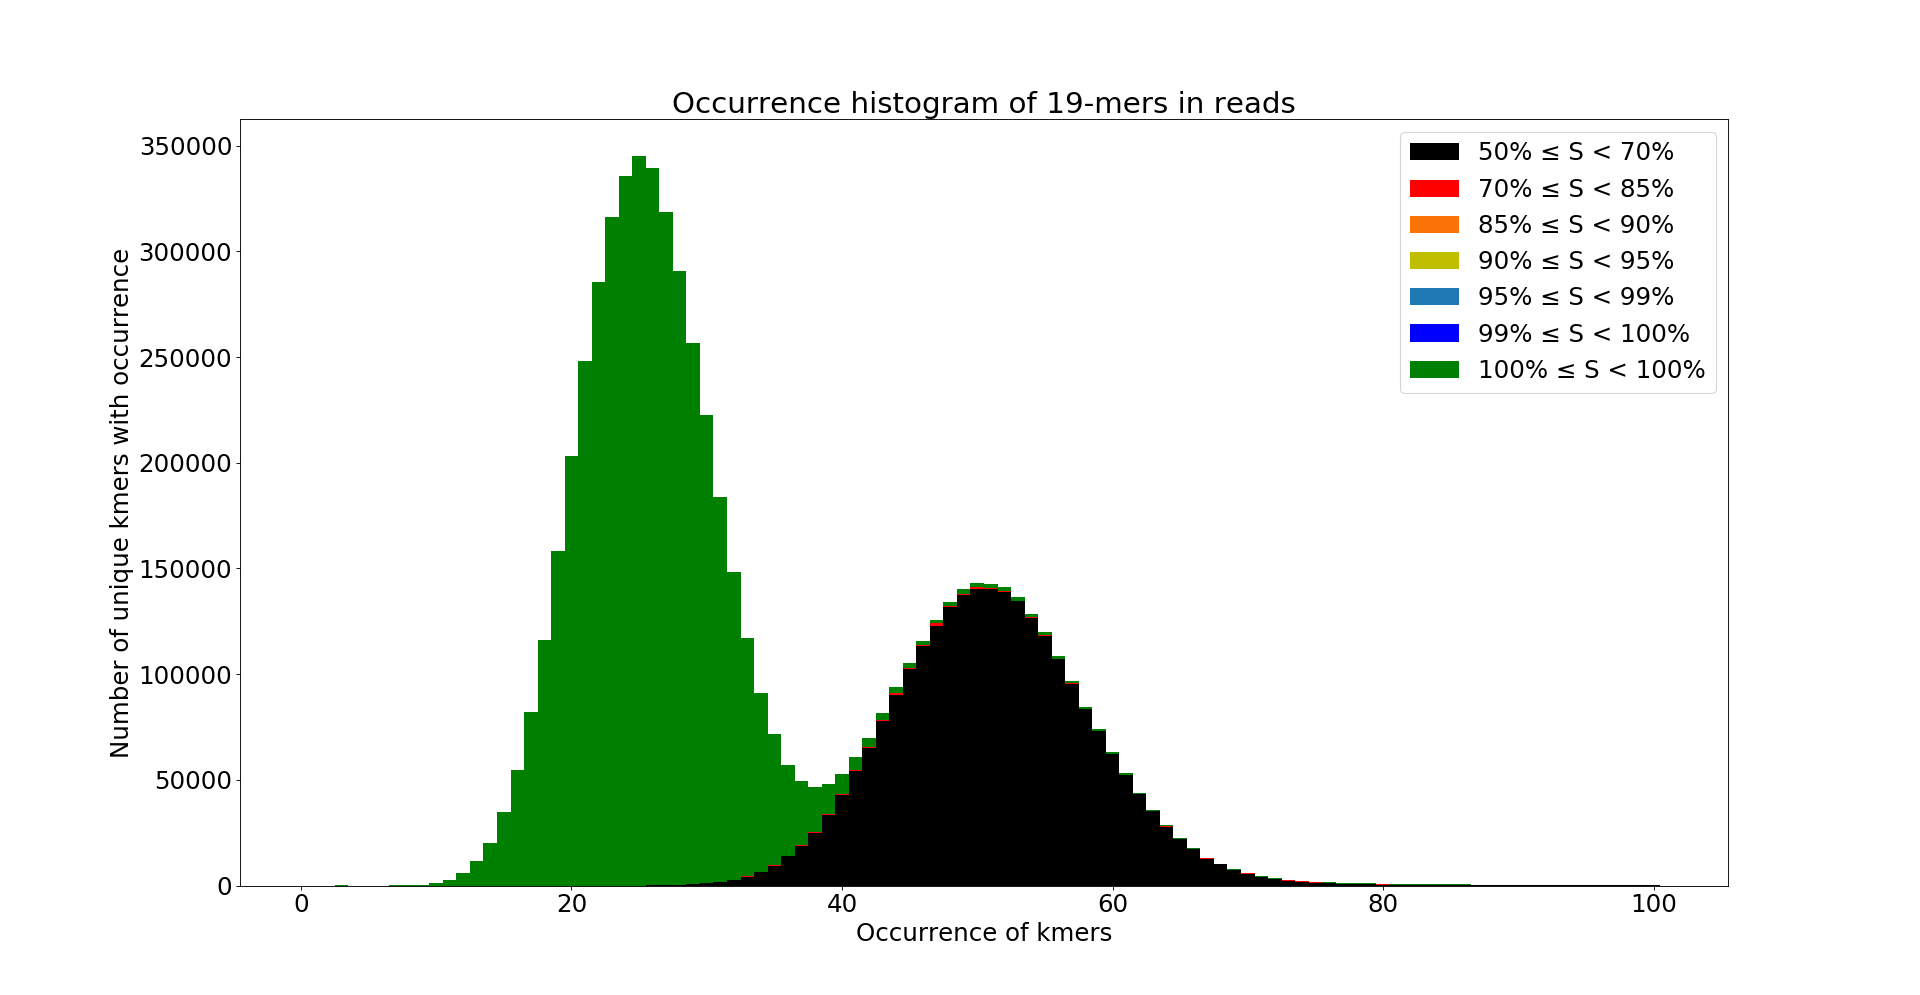
\includegraphics[width=400bp]{figures/19mers.png}
\caption{$k$-mer histogram of EIL30 dataset with k=19}
\label{fig:k19}
\end{figure}

The percentages in the histogram legends describe what proportion of a particular $k$-mers occurrences belong to one of the haplotypes. Every percentage lower than 100 indicates a $k$-mer that occurrs in both haplotypes.


\section{Computation of histogram}

In order to obtain $k$-mer occurrence data, we use Jellyfish\cite{marccais2011fast} counting and dumping tools. Knowing how many times each $k$-mer occurs in the reads, we can compute the histogram. All that remains is to identify the occurrence values resulting in the two peaks, and determining the range of occurrences that we take as a boundary for selecting $k$-mers which we assume to be discriminative. From now on, we will refer to this set of assumed discriminative $k$-mers as suspected discriminative $k$-mer set (or SDK set for brevity).

In our experiments taking $k$-mers that occur between five times and $P$-times, where $P$ is the number of occurrences at the height of the leftmost peak yielded a good tradeoff between the total number of $k$-mers exported and the ratio of their contamination. 

For EIL30 dataset, the selected occurrence range is 10 to 25, resulting in $2221830$ SDKs of which $2221512$ are discriminative.

\begin{figure}
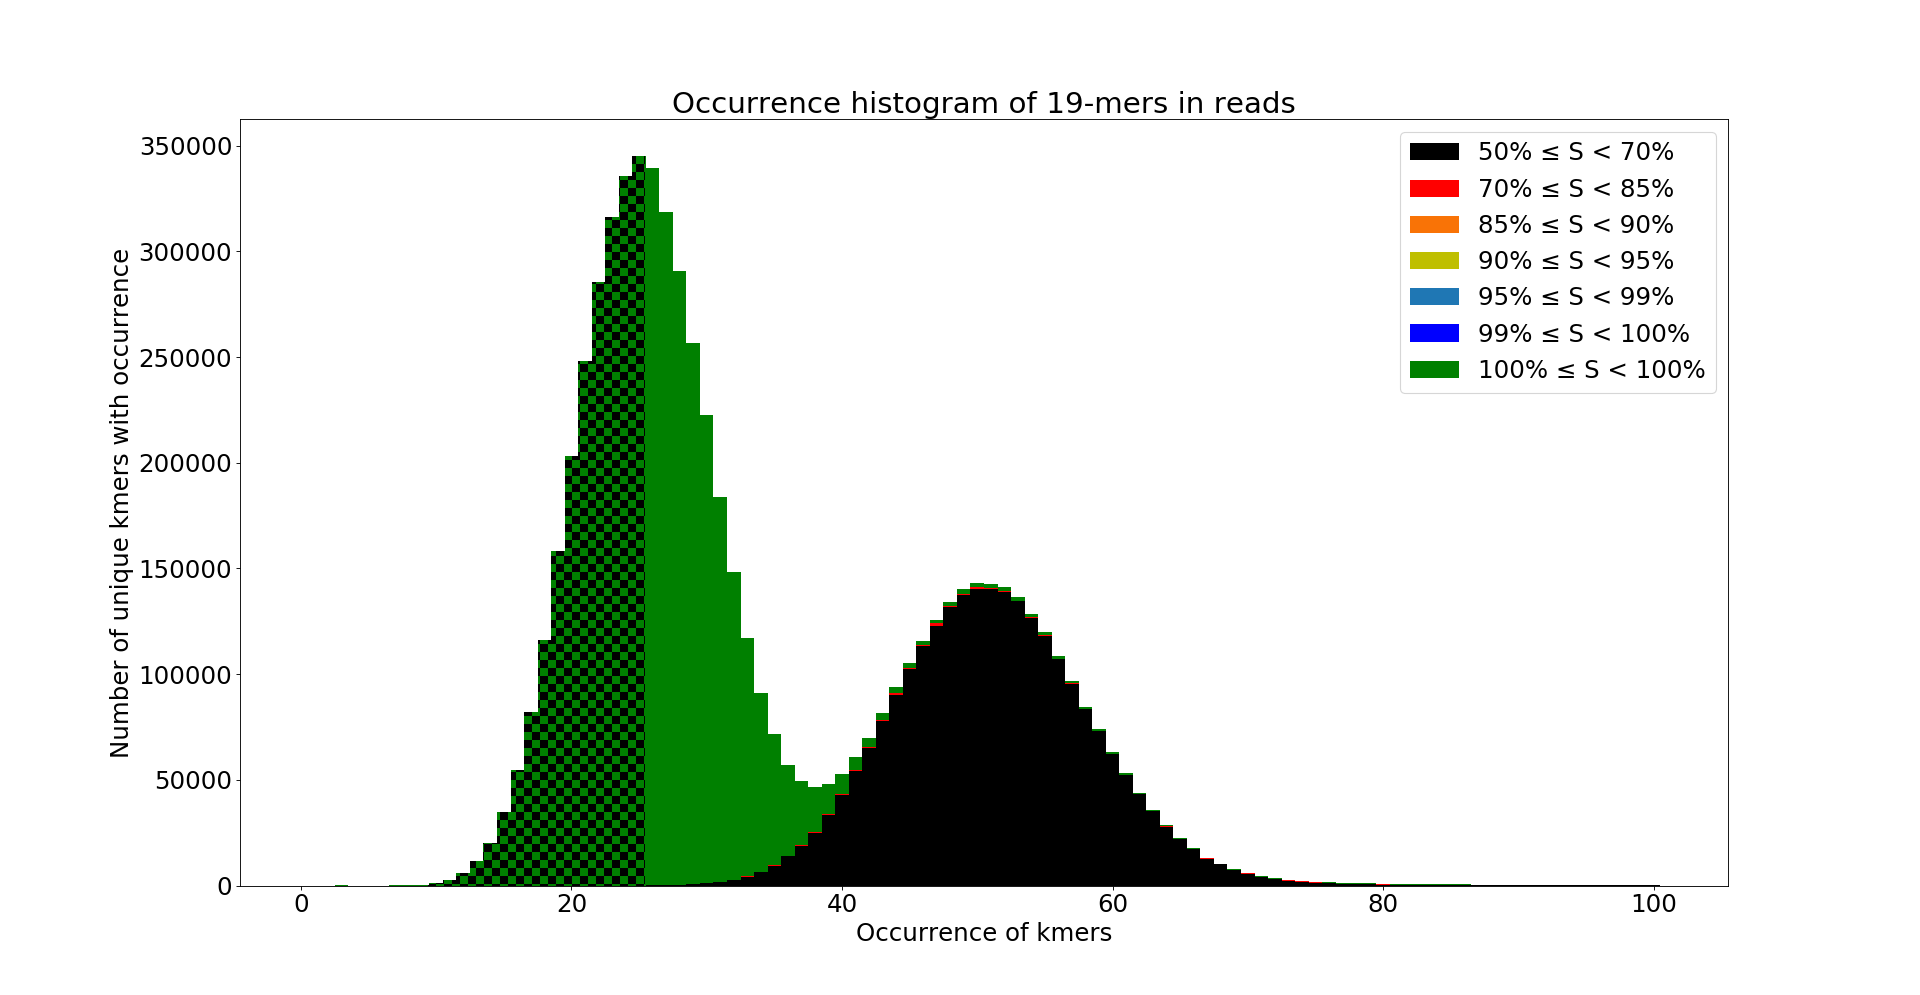
\includegraphics[width=400bp]{figures/19mers_highlighted.png}
\caption{$k$-mer histogram of EIL30 dataset with k=19 and exported SDKs highlighted by checkerboard}
\label{fig:k19_highlighted}
\end{figure}

\section{Discriminative $k$-mer contamination}

As can be seen from figure \ref{fig:k19}, not all $k$-mers with occurrence lower or equal to half the coverage are discriminative. There is some contamination caused by $k$-mers that should reside in the peak on the right, but due to sequencing errors and separation of nucleotides caused by read ends had their occurrences lowered enough to land in the leftmost peak. Contamination of this kind is even more prominent in the case of Nanopore/PacBio reads, as can be seen on the figure \ref{fig:nanopore_hist}. This fact, along with the practical computation of optimal k-value makes Illumina reads a requirement.

\begin{figure}
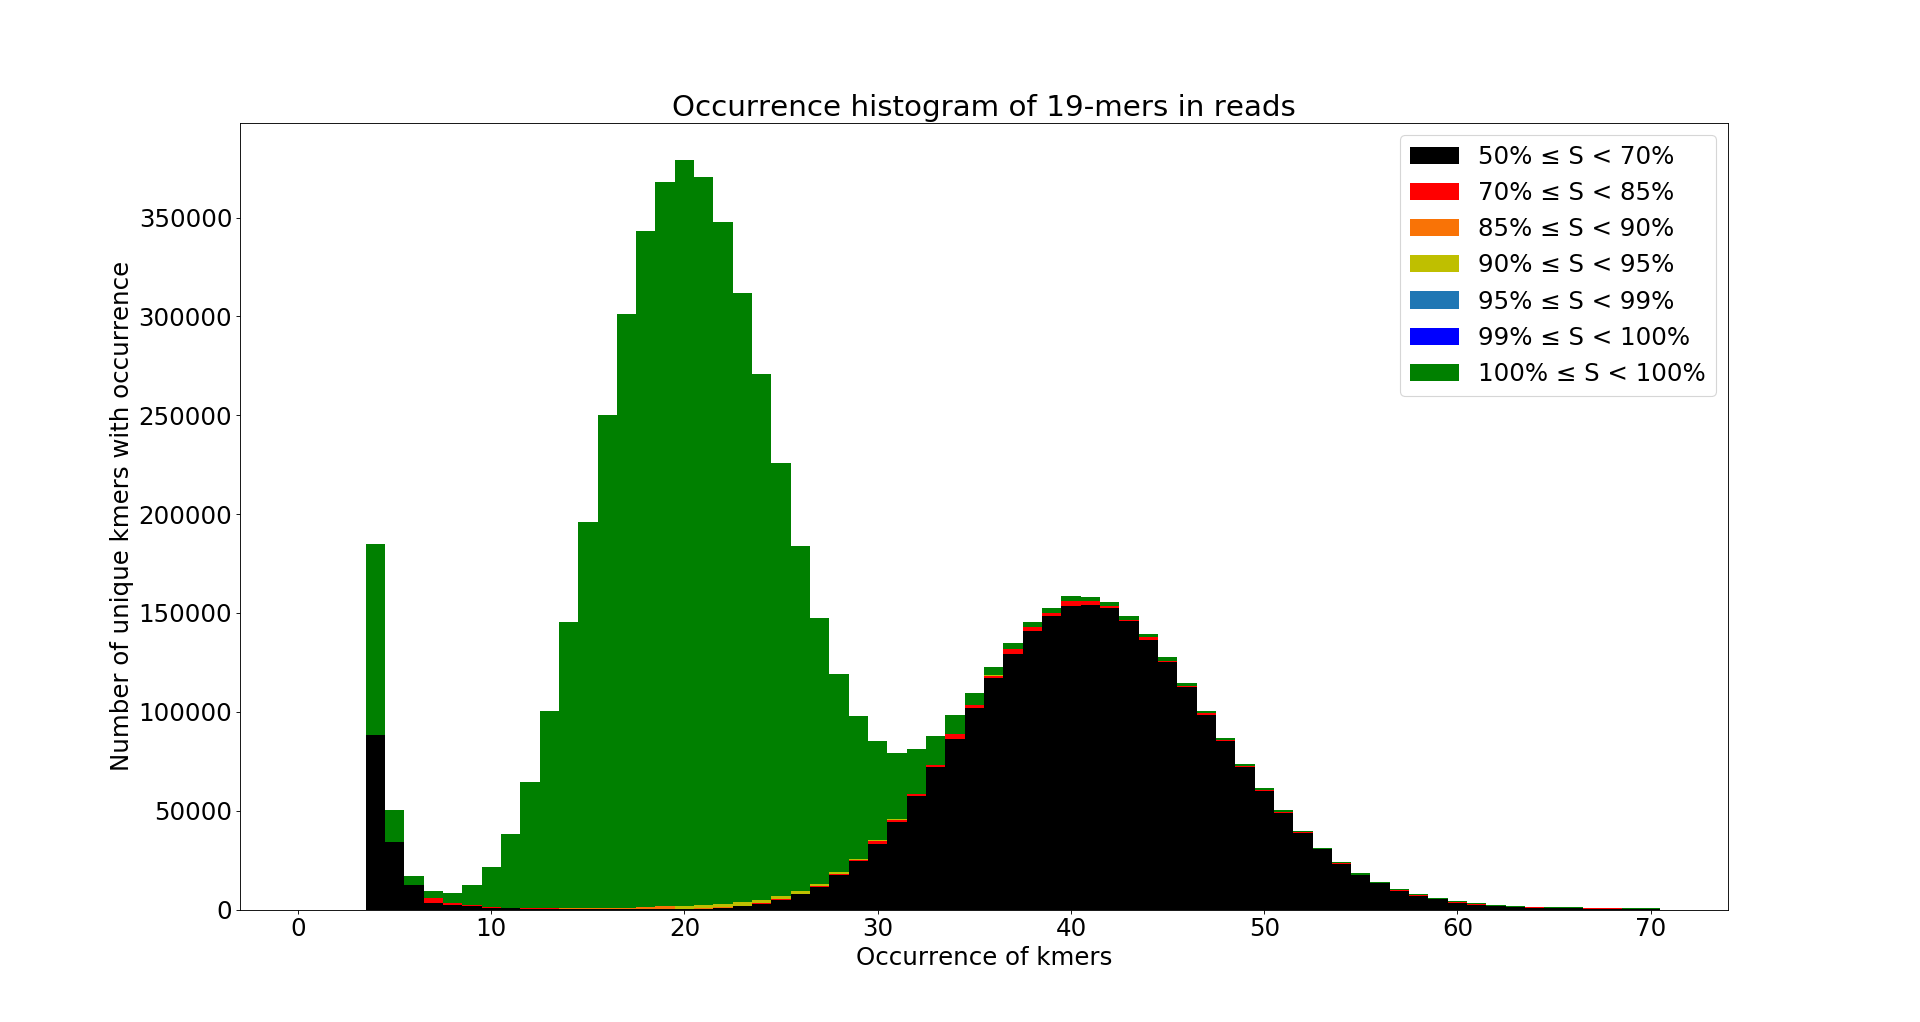
\includegraphics[width=400bp]{figures/nanopore_hist.png}
\caption{$k$-mer histogram of ENP75 dataset. There is noticeable contamination in the left peak.}
\label{fig:nanopore_hist}
\end{figure}

It is necessary to keep the rate of contamination as low as possible early on, as applying the SDKs on reads with higher error rate will increase it further by turning discriminative $k$-mers into contaminants through spurious occurrences caused by sequencing errors. For instance, while the exported SDK set for EIL30 has less than 0.1\% of contaminating $k$-mers, the same set yields 5.6\% contamination in the context of ENP75 dataset.